For that reason, the app was tested by a user outside of the workgroup. Instructions were given to him so that he could understand the concept to navigate through the user-friendly app and report any bugs or challenges faced when performing the following steps:

Step 1) Introduce the user to the last version of the android application: RFCAR app, after instructions given by one of the developers.
%
\begin{figure}[!hbt]
\centering
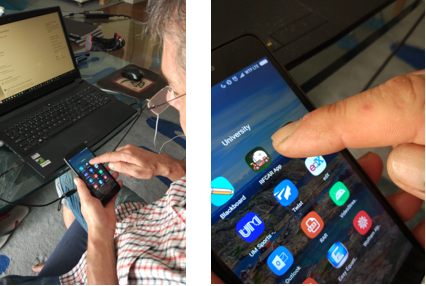
\includegraphics[width=0.8\textwidth]{img/val1.png}
\caption{\label{fig:val1}The final version of the app is launched}
\end{figure}
%

Step 2) When prompted by a system message pop up telling to turn on Bluetooth, turn on Bluetooth.
%
\begin{figure}[!hbt]
\centering
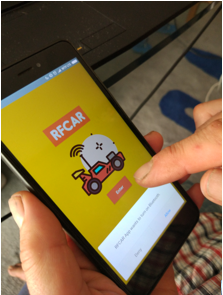
\includegraphics[width=0.3\textwidth]{img/val2.png}
\caption{\label{fig:val2}Bluetooth is enabled, then Enter button is pressed}
\end{figure}
%

Step 3) Press Enter Button. Now, on the main menu, where a idle message, youtube icon and an arcade controller appears, press the button on the top left corner.
%
\begin{figure}[!hbt]
\centering
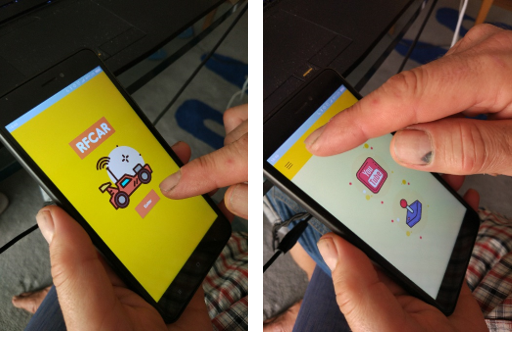
\includegraphics[width=0.5\textwidth]{img/val3.png}
\caption{\label{fig:val3}On main menu, press the top left corner button to open options tab}
\end{figure}
%

Step 4) Press the Bluetooth Discover button to allow the smartphone to be visible to other devices. Press Allow when prompted by the system message.
%
\begin{figure}[!hbt]
\centering
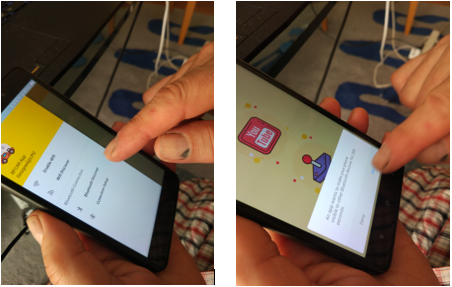
\includegraphics[width=0.5\textwidth]{img/val4.png}
\caption{\label{fig:val4}Bluetooth Discover is pressed, turning the smartphone visible to other devices}
\end{figure}
%

Step 5) Press the Connection Setup button on the lateral sliding tab.
%
\begin{figure}[!hbt]
\centering
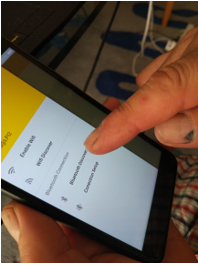
\includegraphics[width=0.3\textwidth]{img/val5.png}
\caption{\label{fig:val5}Connection Setup is pressed to configure Bluetooth connection}
\end{figure}
%

Step 6) Press the Scan Devices button and wait until the Bluetooth enabled target device appears on Discovered Devices subsection and press it. If the target device to pair with doesn't appear, turn on its Bluetooth. A message to conclude the pair phase should appear on both device with a corresponding PIN. Certificate that the PINs match and then click allow and yes on both devices to conclude this stage.
%
\begin{figure}[!hbt]
\centering
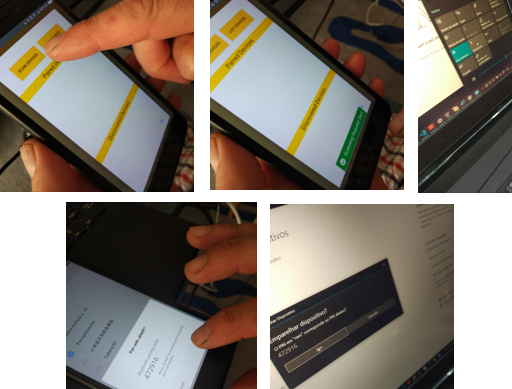
\includegraphics[width=0.8\textwidth]{img/val6.png}
\caption{\label{fig:val6}Scan devices button is pressed, the desired target device to pair with is touched, and the pair phase concludes after the user verify that the PIN of the two devices matches and press yes on both messages displayed on each device}
\end{figure}
%

Step 7) Press the List Devices button and wait again until the target device appears on Paired Devices subsection and press it to establish the connection. 
%
\begin{figure}[!hbt]
\centering
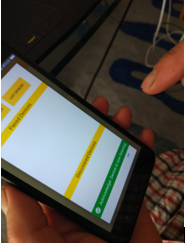
\includegraphics[width=0.3\textwidth]{img/val7.png}
\caption{\label{fig:val7}A connect request is sent and shortly after accepted by the target device}
\end{figure}
%

Step 8) On the sliding tab, press Enable Wifi to turn it on. The device tries to automatically connect to a given Wifi network. If that happens, skip to step 10.
%
\begin{figure}[!hbt]
\centering
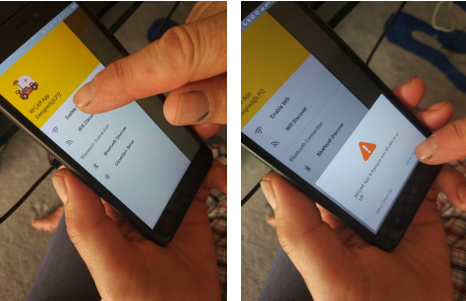
\includegraphics[width=0.5\textwidth]{img/val8.png}
\caption{\label{fig:val8}Enable Wifi button is pressed}
\end{figure}
%

Step 9) Go to main menu and press the Wifi Discovery button and select the desired wireless network on the Wifi Devices section. Touch Wifi Msg to send an initial message to that network to initiate connection. Input the password if prompted.
%
\begin{figure}[!hbt]
\centering
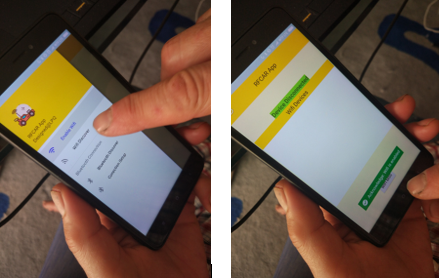
\includegraphics[width=0.5\textwidth]{img/val9.png}
\caption{\label{fig:val9}The desired network is selected after pressing Wifi discover button}
\end{figure}
%

Step 10) Touch the main menu. A full-screen youtube window and some accelerometer statistics emerges corresponding to speed and wheel tilt relative to its maximum values. Touch the play button and tilt the phone to see that the values are passing to the other Bluetooth device.
%
\begin{figure}[!hbt]
\centering
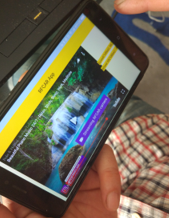
\includegraphics[width=0.3\textwidth]{img/val10.png}
\caption{\label{fig:val10}The application sends accelerometer values to the desired device when phone tilts, and a video feed is enabled}
\end{figure}
%


